\section{Chapter 3}

Neural network can be expressed as a function. For example, it should be able to:
\begin{itemize}
	\item Receive voice signal and output a transcription file.
	\item Receive image and output a text caption.
	\item Receive game state and output a next move.
\end{itemize}

\hfill\break
However, these input has to be represented in a form of numerical unit.

\begin{figure}[H]
	\centering
	\begin{tikzpicture}	
		\node [draw,
		fill=Goldenrod,
		minimum width=2cm,
		minimum height=1.2cm,
		]  (nnet) at (0, 0) {Neural Net};
		
		\node [draw,
		minimum width=2cm,
		minimum height=1.2cm,
		left=2cm of nnet
		]  (input_0) {$[x_1, x_2, ... x_n]$};
				
		\draw[-stealth] (input_0.east) -- (nnet.west) 
		node[midway] (input_center) {}
		node[near end, above] {input};
				
		\node [draw,
		minimum width=2cm,
		minimum height=1.2cm,
		above=of input_0
		]  (input_1) {$x$};
		
		\node [draw,
		minimum width=2cm,
		minimum height=1.2cm,
		below=of input_0
		]  (input_2) {$\begin{pmatrix}
				a & b & c\\ 
				d & e & f
			\end{pmatrix}$};
		
		
		\draw (input_1.east) -- ++(0.5,0) |- (input_center);
		\draw (input_2.east) -- ++(0.5,0) |- (input_center);
		
		%% output
		\node [draw,
		minimum width=2cm,
		minimum height=1.2cm,
		right=2.5cm of nnet
		]  (output_0) {$\{0, 1\}$};
		
		\node [draw,
		minimum width=2cm,
		minimum height=1.2cm,
		above = of output_0
		]  (output_1) {$\begin{pmatrix}
				a & b & c\\ 
				d & e & f
			\end{pmatrix}$};
		
		\node [draw,
		minimum width=2cm,
		minimum height=1.2cm,
		below = of output_0
		]  (output_2) {$[x_1, x_2, ... x_n]$};
		
		\node [draw,
		minimum width=2cm,
		minimum height=1.2cm,
		below = of output_2
		]  (output_3) {$x$};
		
		\draw[-stealth] (nnet.east) -- ++(1.5,0) |- (output_1.west);
		\draw[-stealth] (nnet.east) -- ++(1.5,0) |- (output_2.west);
		\draw[-stealth] (nnet.east) -- ++(1.5,0) |- (output_3.west);
		\draw[-stealth] (nnet.east) -- (output_0.west)
			node[near start, above]{output};		
	\end{tikzpicture}
\end{figure}

\begin{figure}[H]
	\centering
	\begin{tikzpicture}
		\node[draw,
		minimum width=3cm,
		minimum height=1.2cm] at (0, 0) (input_0) {$x$};
		
		\node[draw,
		minimum width=3cm,
		minimum height=1.2cm,
		below=of input_0] (input_1) {$[x_1, x_2, \cdots, x_n]$};
		
		\node[draw,
		minimum width=3cm,
		minimum height=1.2cm,
		below=of input_1] (input_2) {$\begin{bmatrix}
				x_{11} & \cdots & x_{m1}\\ 
				\vdots & \ddots & \vdots\\
				x_{1n} & \cdots & x_{mn}\\
			\end{bmatrix}$};
		
		\coordinate[right=of input_1] (hub_input){};
		\coordinate[right=of input_0] (top_junction){};
		\coordinate[right=of input_2] (bottom_junction){};
		
		\path[-] (input_0.east) edge (top_junction)
			(top_junction) edge[-] (hub_input)
			(input_2.east) edge (bottom_junction)
			(bottom_junction) edge[-] (hub_input);
			
		\node [draw,
		fill=Goldenrod,
		minimum width=2cm,
		minimum height=1.2cm,
		right=2cm of hub_input]  (nnet) {Neural Net};
		
		\path[-] (input_1.east) edge (hub_input)
			(hub_input) edge[->] (nnet.west);
			
		\coordinate[right=of nnet] (hub_output){};
			
		\node[draw,
		minimum width=3cm,
		minimum height=1.2cm,
		above right=of hub_output] (output_1) {$x$};
		
			\node[draw,
		minimum width=3cm,
		minimum height=1.2cm,
		above right =of output_0] (output_0) {$x$};
		
	\end{tikzpicture}
\end{figure}

\subsection{The original perceptron model.}

\begin{figure}[H]
	\centering
	
	\begin{tikzpicture}
		
		\node[draw,
		circle,
		minimum size=0.6cm,
		fill=Rhodamine!50
		] (sum) at (0,0){};
		
		\node [draw,
		fill=Goldenrod,
		minimum width=2cm,
		minimum height=1.2cm,
		right= 2cm of sum
		]  (threshold) {$T$};
		
		\draw[-stealth] (sum.east) -- (threshold.west) 
		node[midway,above]{sum};
		
		\draw[-stealth] (threshold.east) -- ++(2, 0) 
		node[midway,above]{output};
	\end{tikzpicture}
\end{figure}

\hfill\break
If we are modelling these functions as neural network, there are some questions that need to be answered:
\begin{itemize}
	\item How do we represent the input?
	\item How do we represent the output?
	\item How do we compose the network that performs the requisite function?
\end{itemize}

\hfill\break
In what we have seen so far, neural network is composed of number of simple elements called perceptrons. On individual level, each perceptron has:
\begin{itemize}
	\item Bunch of real value input.
	\item Bias term.
\end{itemize}

\begin{figure}[H]
	\centering
	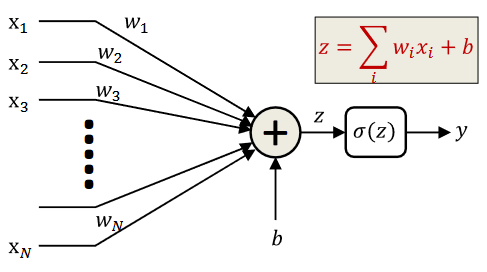
\includegraphics[width=0.5\textwidth]{3_perceptron}
\end{figure}

\hfill\break
The perceptron first compute the affine function of the inputs which is the weighted sum of the individual inputs plus the bias term $b$, giving us value $Z$. This affine value $Z$ get put through an activation function $\sigma(Z)$

\begin{figure}[H]
	\centering
	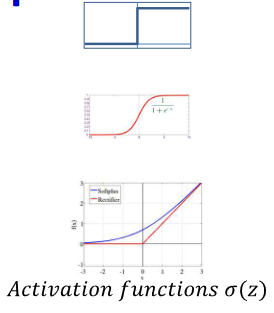
\includegraphics[width=0.5\textwidth]{3_activation_function}
\end{figure}

\hfill\break
The parameter of the perceptron, which determine how it behaves are the weights
$w$ and the bias $b$. The bias term is usually isolated with the inputs, however
there is a different way in viewing the bias term, which is to say that we can
augment the input with an additional component whose value is $1$. If we do so,
then the weight of this additional input, $w_{N+1}$ effectively capture the
bias.

This is just a matter of representation. Say if the perceptron does not
explicitly showing a bias, then we must understand that we are considering that
the input has been augmented by the additional term such that the input is $1$ and
the weight $w_{N+1}$ is the bias.

\begin{figure}[H]
	\centering
	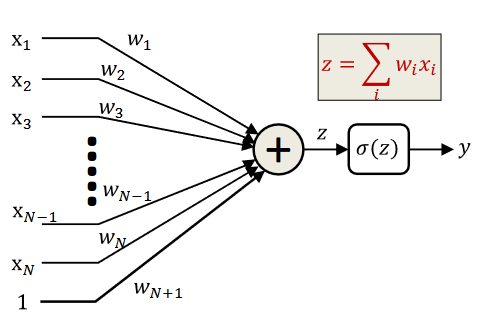
\includegraphics[width=0.5\textwidth]{3_perceptron_wo_bias}
\end{figure}


